\section{Metodología}

Para llevar a cabo el desarrollo del prototipo se utilizó la metodología Modelo de Prototipos, debido a que no solo va dirigido al hardware sino también al software, esto permite obtener objetivos específicos y es de gran utilidad para el manejo de datos aportados y su manipulación. \\

El modelo de prototipos permite que todo el sistema, o algunos de sus partes se construyan rápidamente para comprender con facilidad y aclarar ciertos aspectos en los que se aseguren que el desarrollador, el usuario y el cliente estén de acuerdo en lo que se necesita, así como también la solución que se propone para dicha necesidad y de esta forma minimizar el riesgo y la incertidumbre en el desarrollo. Este modelo se encarga del desarrollo de diseños para que estos sean analizados y prescindir de ellos a medida que se adhieran nuevas especificaciones, es ideal para medir el alcance del producto. \\

El modelo principalmente se aplica cuando un cliente define un conjunto de objetivos generales para el software, es decir, se tiene en claro la idea principal del sistema a desarrollar, pero no se cuenta con la delimitación ni los detalles de dicho sistema, como los son: los requisitos de entrada, procesamiento y salida, por lo cual la creación de los prototipos ayuda al cliente a entender de mejor manera cuál será el resultado de la construcción cuando los requisitos estén satisfechos \cite{cuarenta}. \\

\begin{figure}[h]
	\centering
	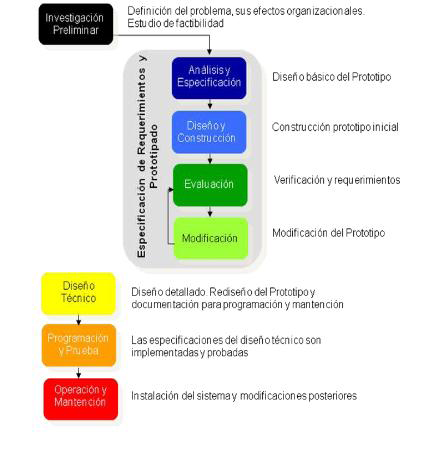
\includegraphics[scale=0.75]{analisis/imagenes/modelo_prototipos}
	\textbf{\caption{\small{Modelo de Prototipos \cite{cuarenta}.}}}
	\label{Seccion2:Figura2.1}
\end{figure}

A continuación, se presenta el enfoque paso a paso para diseñar un prototipo: \\

\begin{itemize}
	\item \textbf{Identificación del requisito básico:} Este paso implica la comprensión de los requisitos más básicos de productos, especialmente en términos de interfaz de usuario. Los más intrincados detalles del diseño interno y aspectos externos como el rendimiento y la seguridad pueden ser ignorados en esta etapa.
	\item \textbf{El desarrollo del prototipo inicial:} El prototipo inicial se desarrolla en esta etapa, donde se exhiben los requisitos muy básicos y se proporcionan interfaces de usuario. Estas características pueden no funcionar exactamente de la misma manera internamente en el software real desarrollado y las soluciones se utilizan para dar la misma apariencia que el cliente en el prototipo desarrollado.
	\item \textbf{Revisión del Prototipo:} El prototipo desarrollado se presenta a continuación para el cliente y los otros actores importantes en el proyecto. La retroalimentación se recoge de una manera organizada y se utiliza para mejoras adicionales en el producto en fase de desarrollo.
	\item \textbf{Revisar y mejorar el Prototipo:} La retroalimentación y los comentarios de revisión se discuten en esta etapa y algunas negociaciones ocurren con el cliente en función de factores como, el tiempo y las limitaciones presupuestarias y la viabilidad técnica de la implementación real.
\end{itemize}

Los cambios aceptados se incorporan de nuevo en el nuevo prototipo desarrollado y el ciclo se repite hasta que se cumplan las expectativas del cliente \cite{cuarentayuno}. \\

Por lo tanto, en el siguiente diagrama trataremos de describir a detalle las fases enfocadas a nuestro proyecto utilizando la metodología de prototipos.

\begin{figure}[h]
	\centering
	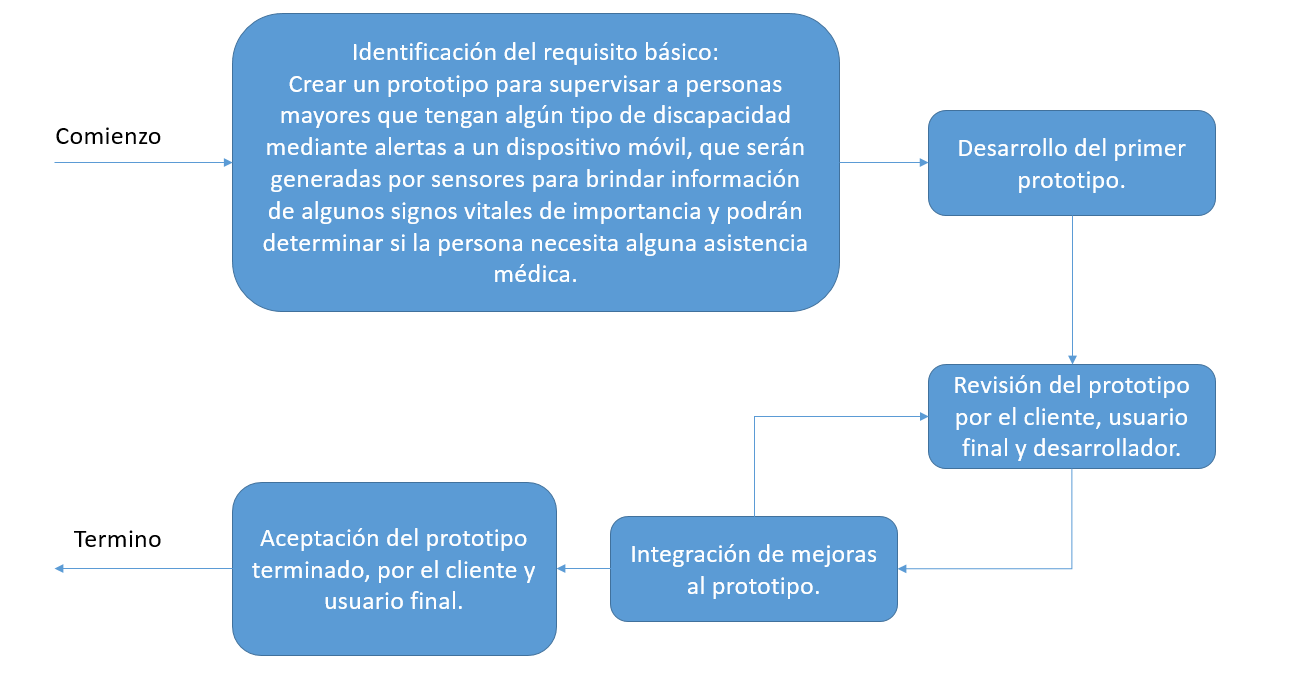
\includegraphics[scale=0.35]{analisis/imagenes/diagrama_prototipo}
	\textbf{\caption{\small{Diagrama para la realización del proyecto utilizando la metodología de prototipos.}}}
	\label{Seccion2:Figura2.2}
\end{figure}